\documentclass{beamer}

\usepackage[utf8]{inputenc}
\usepackage{hyperref}

\usetheme{Berkeley}
\beamertemplatenavigationsymbolsempty
\setbeamertemplate{headline}{}
 
\title{Tracing in FoodChain-Lab}
\date{}
 
\begin{document}
\maketitle

\section{Tasks}
\begin{frame}
	\begin{itemize}
		\item Use the example workflow from \url{https://github.com/SiLeBAT/BfROpenLabResources/raw/master/GitHubPages/workflows/FCL_Example.zip}.
		\item Visualize the forward and backward trace of a station via the \textbf{Tracing View}.
		\item Deactivate "Cross Contamination" for the black station and see how the trace changes.
	\end{itemize}
\end{frame}
 
\section{1}
\begin{frame}
	\begin{center}
  		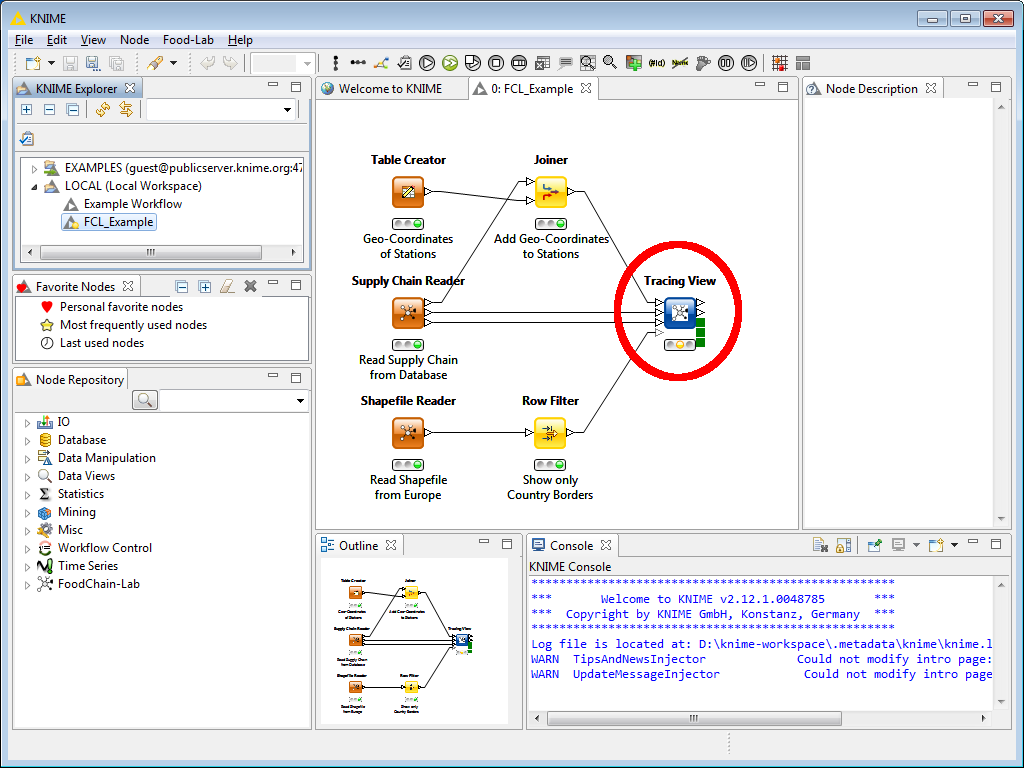
\includegraphics[height=0.6\textheight]{1.png}
	\end{center}
	\begin{itemize}
		\item Import the Example Workflow from \url{https://github.com/SiLeBAT/BfROpenLabResources/raw/master/GitHubPages/workflows/FCL_Example.zip}.
		\item Open the \textbf{Tracing View} by double-clicking on it.
	\end{itemize}
\end{frame}

\section{2}
\begin{frame}
	\begin{center}
  		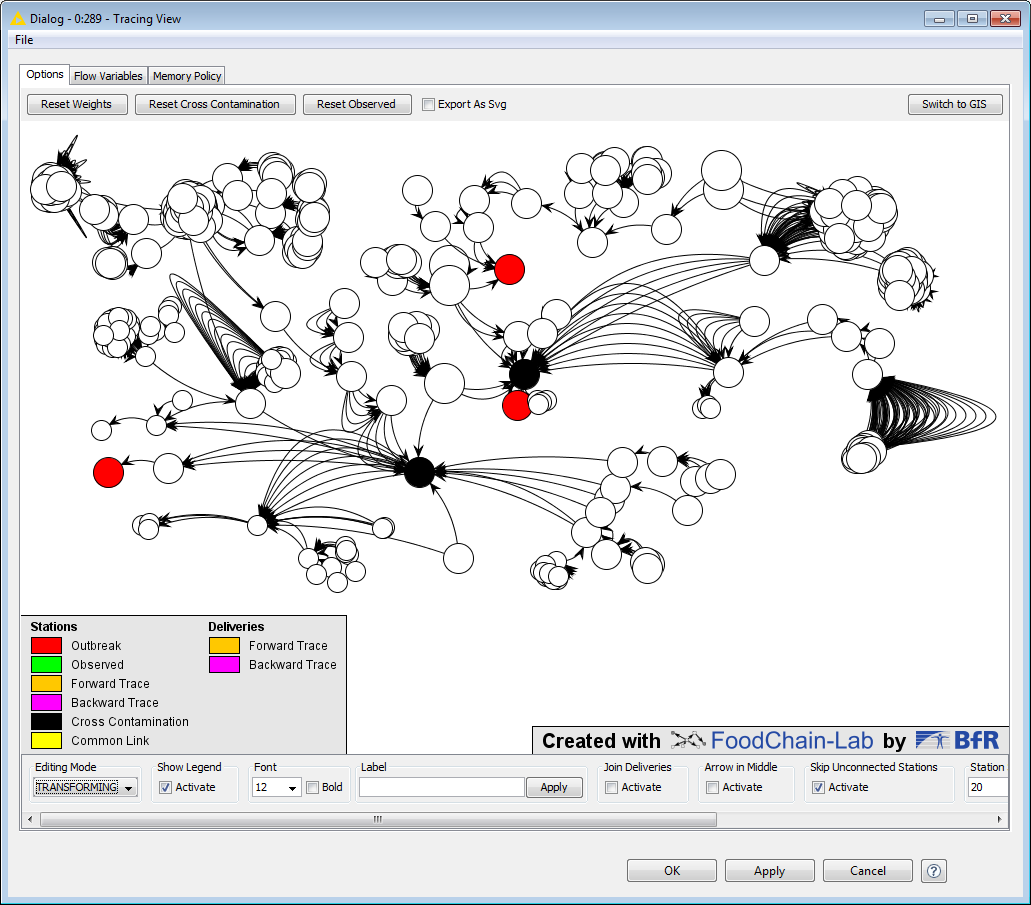
\includegraphics[height=0.6\textheight]{2.png}
	\end{center}
	\begin{itemize}
		\item In the delivery graph you can see 9 \textbf{Outbreak} stations (red) and one station where \textbf{Cross Contamination} is assumed (black).
		\item The size of each station is based on its "Score", which depends on the \textbf{Outbreak} stations that can be reached from the station.
	\end{itemize}
\end{frame}

\section{3}
\begin{frame}
	\begin{center}
  		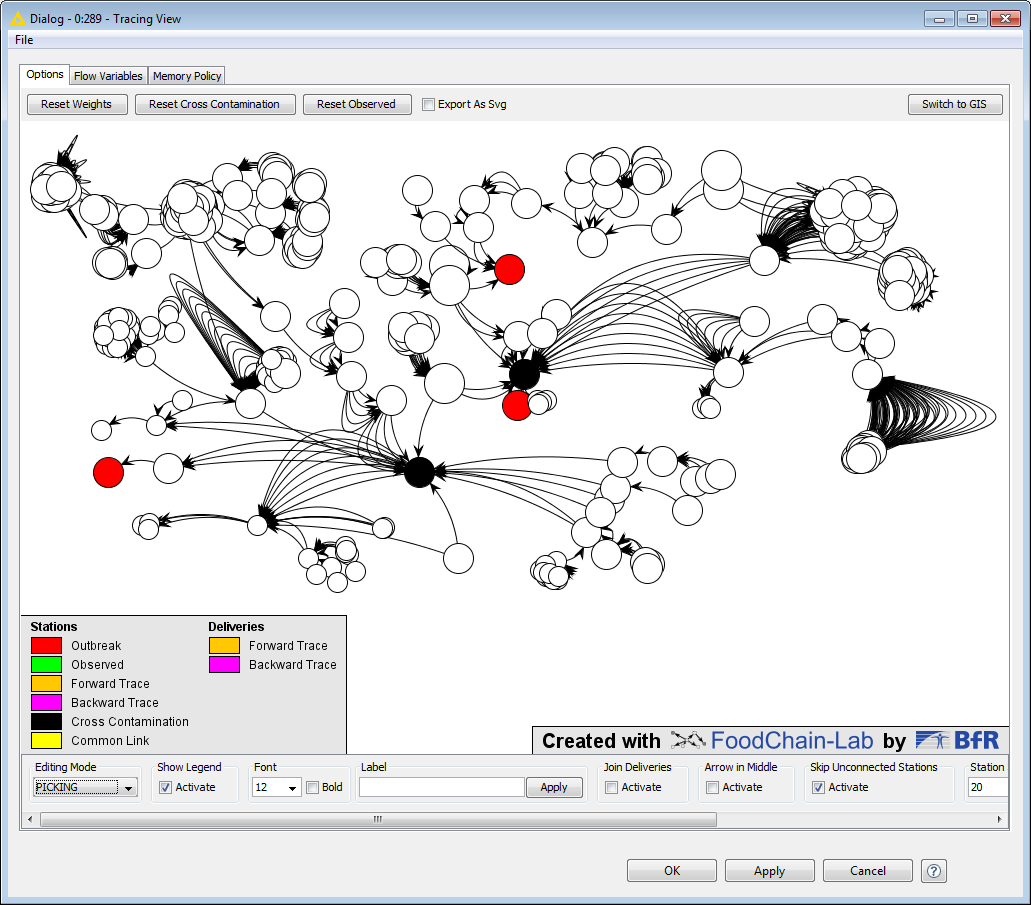
\includegraphics[height=0.6\textheight]{3.png}
	\end{center}
	\begin{itemize}
		\item We will now observe the trace of a single station in detail.
		\item Set "PICKING" as \textbf{Editing Mode} and double click on the station in the red circle.
	\end{itemize}
\end{frame}

\section{4}
\begin{frame}
	\begin{center}
  		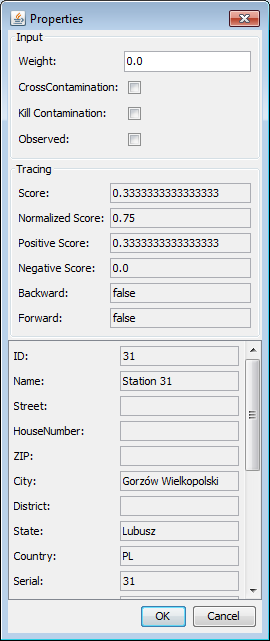
\includegraphics[height=0.6\textheight]{4.png}
	\end{center}
	\begin{itemize}
		\item A dialog will pop up, that all attributes of the station.
		\item Additionally you can change "Weight", "Cross Contamination", "Kill Contamination" and "Observed".		
	\end{itemize}
\end{frame}

\section{5}
\begin{frame}
	\begin{center}
  		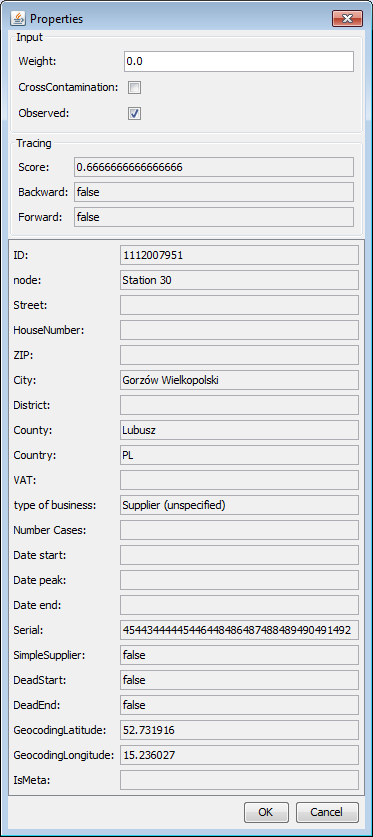
\includegraphics[height=0.6\textheight]{5.png}
	\end{center}
	\begin{itemize}
		\item Select \textbf{Observed} and press \textbf{OK}.
	\end{itemize}
\end{frame}

\section{6}
\begin{frame}
	\begin{center}
  		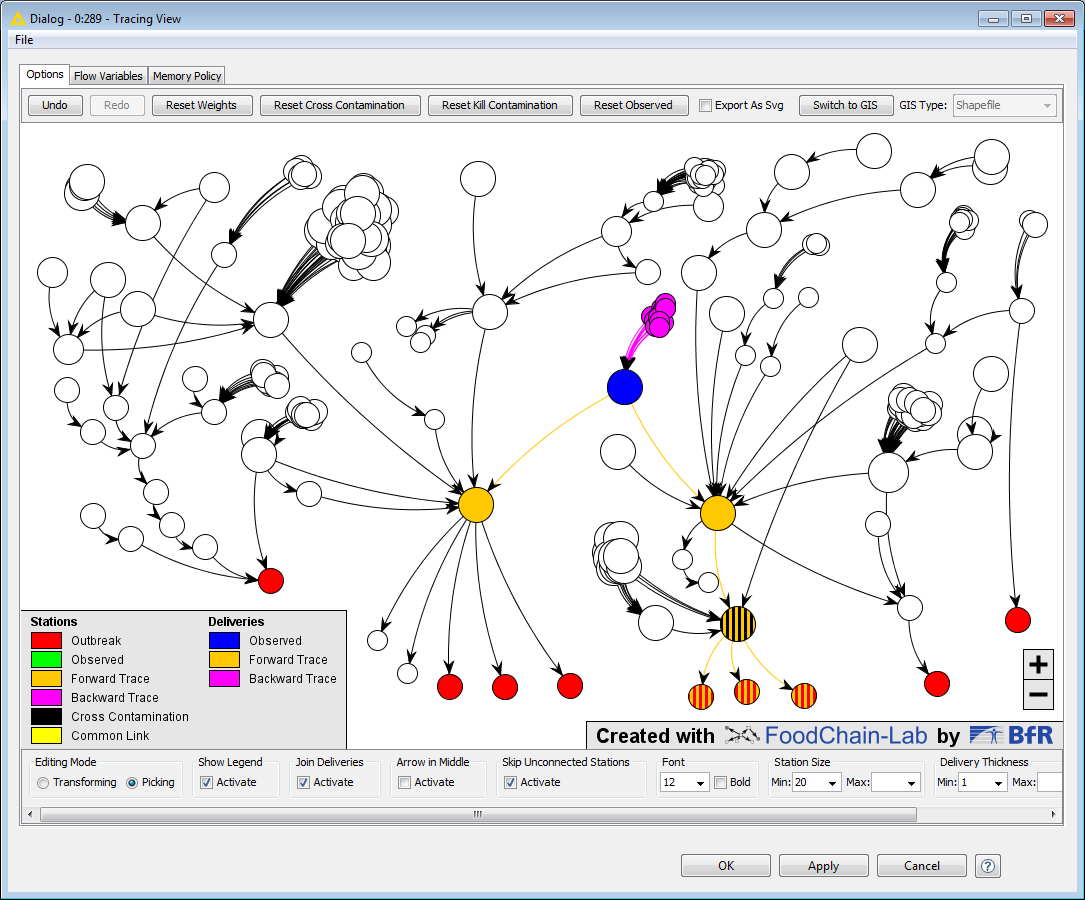
\includegraphics[height=0.6\textheight]{6.png}
	\end{center}
	\begin{itemize}
		\item All stations/deliveries of the forward trace are orange-colored and the ones of the backward trace are purple.
		\item Three \textbf{Outbreak} stations are also orange striped now. That means they are also on the forward trace of the observed station.
	\end{itemize}
\end{frame}

\section{7}
\begin{frame}
	\begin{center}
  		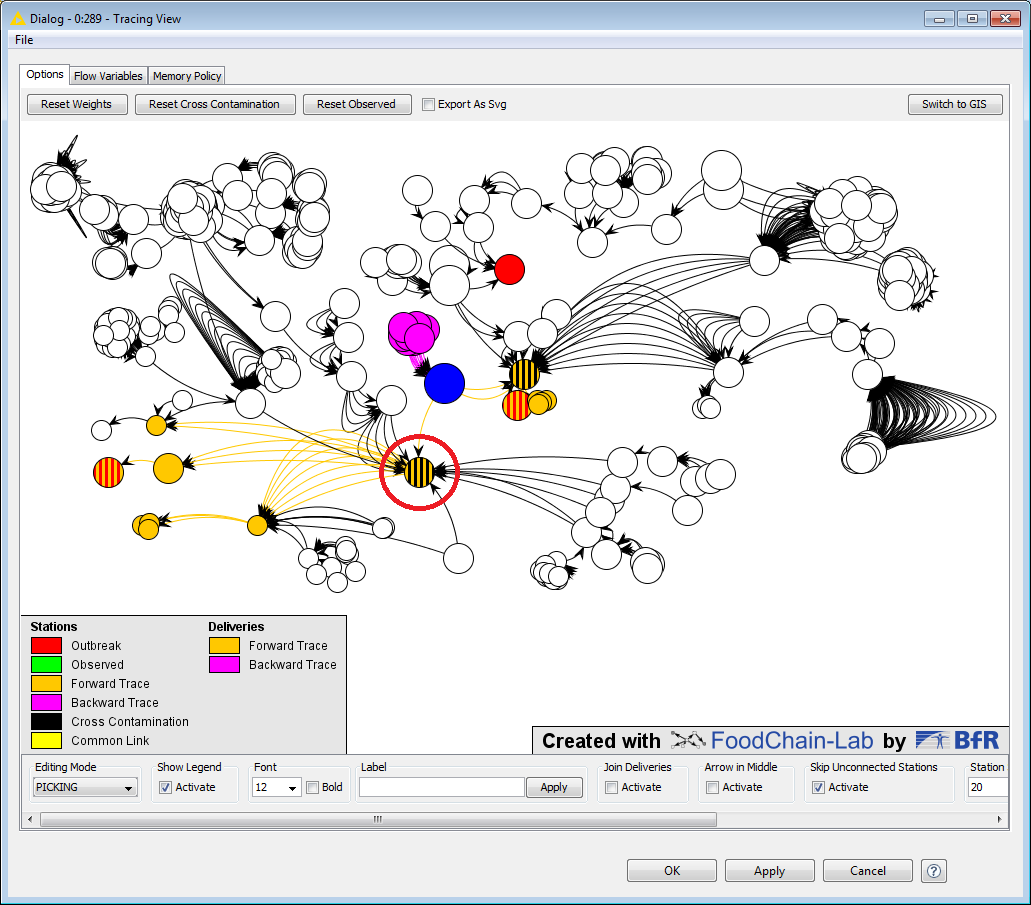
\includegraphics[height=0.6\textheight]{7.png}
	\end{center}
	\begin{itemize}
		\item Let's see what happens if we deactivate cross contamination in the station in the red circle.
		\item So double click on it.
	\end{itemize}
\end{frame}

\section{8}
\begin{frame}
	\begin{center}
  		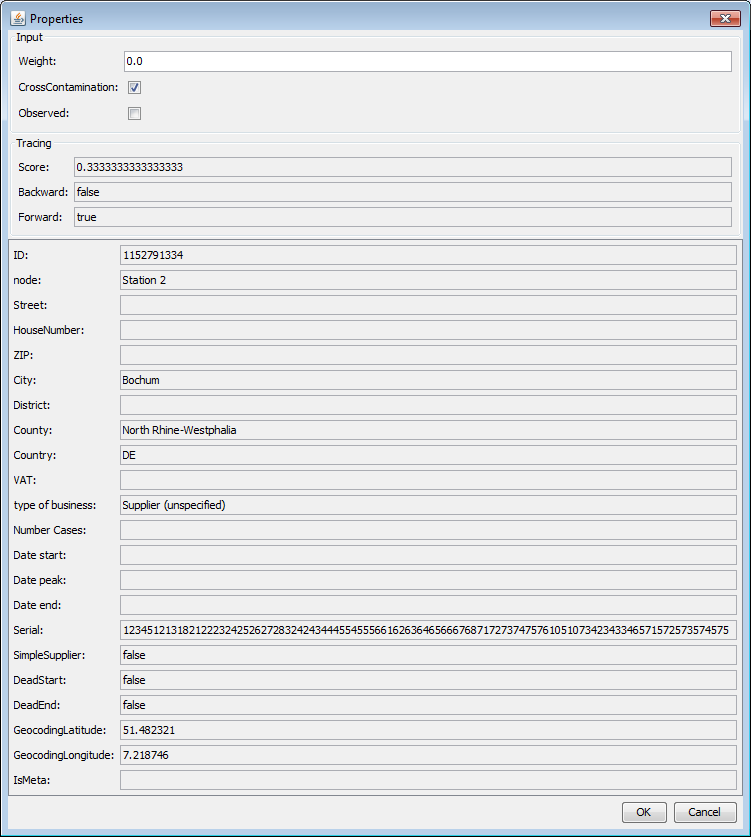
\includegraphics[height=0.6\textheight]{8.png}
	\end{center}
	\begin{itemize}
		\item Uncheck \textbf{CrossContamination} and press \textbf{OK}.
	\end{itemize}
\end{frame}

\section{9}
\begin{frame}
	\begin{center}
  		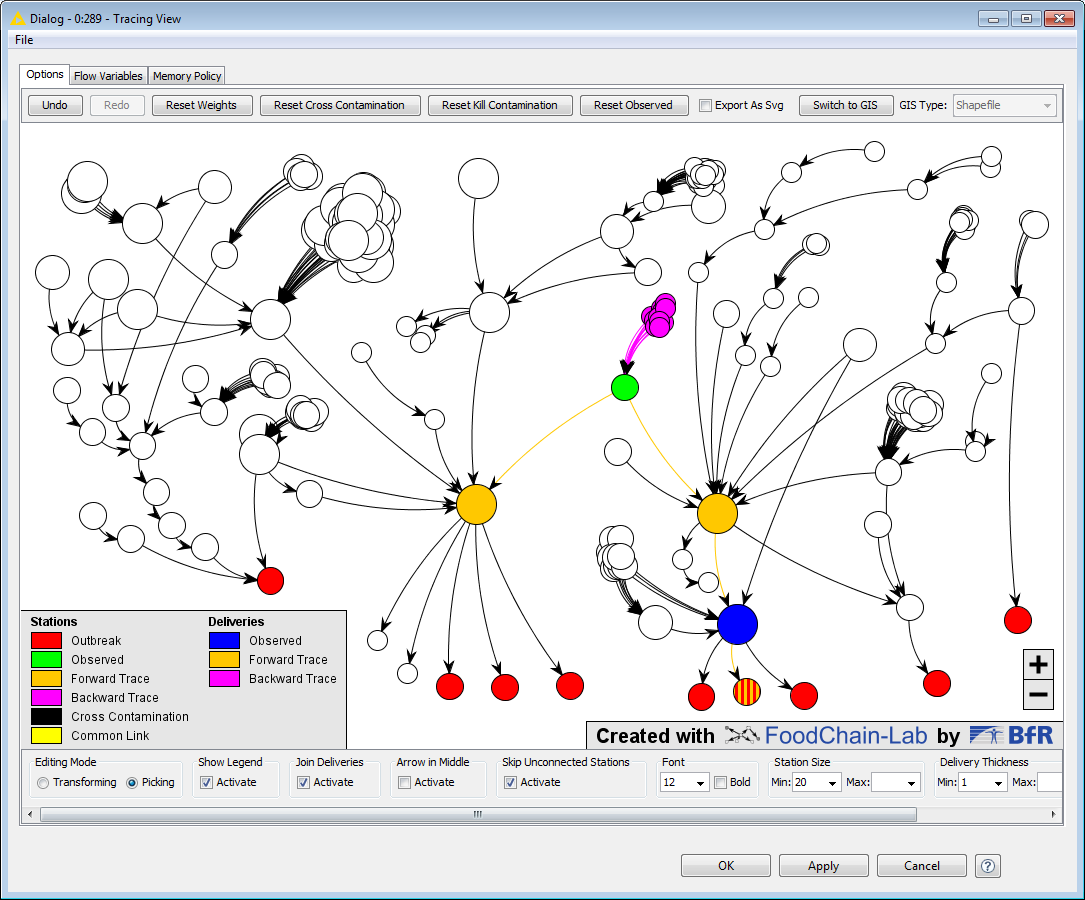
\includegraphics[height=0.6\textheight]{9.png}
	\end{center}
	\begin{itemize}
		\item Deactivating cross contamination changed the forward trace of the observed station.
		\item Now two of \textbf{Outbreak} stations, that were striped before, cannot be reached anymore.
	\end{itemize}
\end{frame}

\end{document}